\section{Algoritmo Goloso}

\subsection{Soluci\'on}

Proponemos una solución heurística golosa para encontrar un conjunto dominante de un grafo lo mas pequeño posible con una complejidad polinomial.\\
Para ello nos basamos en una estrategia de selección de nodos dominantes, la cual consiste en elegir el nodo que mas adyacentes no cubiertas tenga (es decir, que todavía no fueron dominadas) y verificando en cada iteración si el conjunto actual es dominante. En base a diferentes estrategias y tipos de grafos (estrella, bipartitos, completos, estrellas unidas, caminos, ciclos) que fuimos observando, elegimos esta ya que fue la que más nos convenció y mejores resultados nos dió debido a que siempre intenta seleccionar el nodo que mas pueda dominar a otros nodos reduciendo el conjunto de los no cubiertos y acercándose a una mejor solución del problema. 

\subsection{Pseudocódigo}

\begin{codebox}
\Procname{$\proc{MCDGreedy}$ (\textbf{in} $Grafo$)}{conjuntoDomGoloso}{ConjDeVértices}
\li	vértices = lista de vértices del grafo	\RComment O(n)
\li	dominantes = conjunto vacio de vértices	
\li	\textbf{Mientras} no estén TodasCubiertas(vértices) \Do \RComment O($n$)
\li 		Ordeno los vértices por la cantidad adyacentes que tenga no cubiertas (sin dominar), de mayor a menor. \RComment O(n*log(n))
\li 		Elijo como dominante al primero de la lista y lo agrego al conjunto de \textbf{dominantes} \RComment O(n)
\li 		Saco de la lista de vértices al elegido \RComment O(n)
\li 		ActualizarGradoSinDominar(elegido) \RComment Actualizo los nodos del grafo,\\ disminuyendo la cantidad de \textit{grado sin dominar} de los adyacentes al elegido, y de los adyacentes a estos.  O($n^2$)
\End
\li	\textbf{return} dominantes
\end{codebox}

\begin{codebox}
\Procname{$\proc{TodasCubiertas}$ (\textbf{in} $ListaDeVertices$)}{result}{Boolean}
\li 	\textbf{Para todos} los vértices en la lista \Do
\li 		\textbf{Si} el vértice no esta dominado \Do
\li 			\textbf{return} falso \End \End
\li 	\textbf{return} verdadero
\end{codebox}

\begin{codebox}
\Procname{$\proc{ActualizarGradoSinDominar}$ (\textbf{in} $Vertice$ $elegido$)}{}{}
\li 	Marcar al vértice elegido como dominado.
\li 	unionDeAdyacentes = lista de vértices vacía, que luego se usará para actualizar.
\li 	\textbf{Para todos} los vértices en la lista de adyacentes al \textbf{elegido} \Do
\li 		\textbf{Si} el vértice \textit{elegido} no estaba dominado \Do
\li 			Decremento en uno el grado de adyacentes sin dominar del nodo actual \End
\li 		\textbf{Si} el nodo actual \textit{elegido} no estaba dominado \Do
\li 			Agrego los nodos adyacentes a la lista \textit{unionDeAdyacentes} \End
\li 		Marco al nodo actual como dominado. \End
\li 	\textbf{Para todos} los vértices en la lista unionDeAdyacentes \Do 
\li 			Decremento en uno el grado de adyacentes sin dominar del nodo actual \End %\RComment Recorro unionDeAdyacentes para actualizar\\  el grado de nodos adyacentes sin dominar
\end{codebox}

\subsection{Análisis de Complejidad}

La complejidad del algoritmo es de O($n^3$)

El algoritmo comienza creando una lista de vértices en O(n).\\
Luego entra en un ciclo que como máximo será lineal en la cantidad de vértices porque en cada ciclo saca un vértice y la cantidad de vértices es finita. En cada iteración deberá comprobar si el conjunto actual de vértices elegidos domina todo el grafo en O($n$), ordenar todos los vértices en O(n*log(n)) mediante QuickSort, elegir un vértice en O(1), removerlo de la lista en O(n) y finalmente actualizar el atributo de los grados sin dominar adyacentes de cada nodo en O($n^2$), esto es porque para los adyacentes del nodo elegido y a su vez para los adyacentes de estos tengo que bajar en uno este atributo, recorrer los adyacentes me lleva O(n) y por cada adyacente recorrer sus adyacentes también me lleva O(n), O(n) * O(n) = O($n^2$).\\

Por lo tanto, la complejidad nos queda:\\
O(n) + O(n) * (O($n^2$) + O(n*log(n) + O(n) + O($n^2$)) = O($n^3$)\\\\

La complejidad final del algoritmo goloso es de O($n^3$), cumpliendo el objetivo de ser polinomial.

\subsection{Mejor Caso}

Las familias de grafos en donde la solución es la mejor son la de los bipartitos completos, triangulos unidos, estrellas, arboles binarios, arbol de cliques, completo entre filas, hipercubos. Esto es debido al ordenamiento y selección de nodos que realiza nuestra estrategia, obteniendo en cada iteración el nodo justo para lograr el resultado óptimo, ya sea porque contienen un nodo universal o porque selecciona nodos de subgrafos completos maximales.

Decidimos focalizarnos en tres tipos de familias para hacer el análisis (Triangulos Unidos, Árbol de Cliques y Completo entre Filas) por el solo hecho de ser familias átipicas y no muy frecuente analizadas, y que además de dar siempre los mejores casos, se comportan por debajo de la cota de complejidad para este algoritmo.

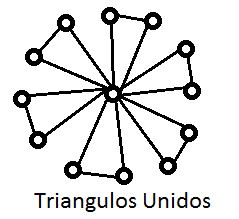
\includegraphics[width=5cm]{./graficos/triangulosunidos.png}
% grafico.eps: 0x0 pixel, 300dpi, 0.00x0.00 cm, bb=50 50 410 302
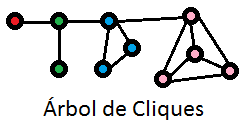
\includegraphics[width=5cm]{./graficos/cliquetree.png}
% grafico.eps: 0x0 pixel, 300dpi, 0.00x0.00 cm, bb=50 50 410 302
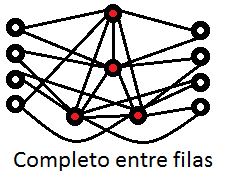
\includegraphics[width=5cm]{./graficos/completoentrefilas.png}
% grafico.eps: 0x0 pixel, 300dpi, 0.00x0.00 cm, bb=50 50 410 302

A continación un gráfico para grafos de hasta 2000 nodos entre las tres familias:

\begin {center}
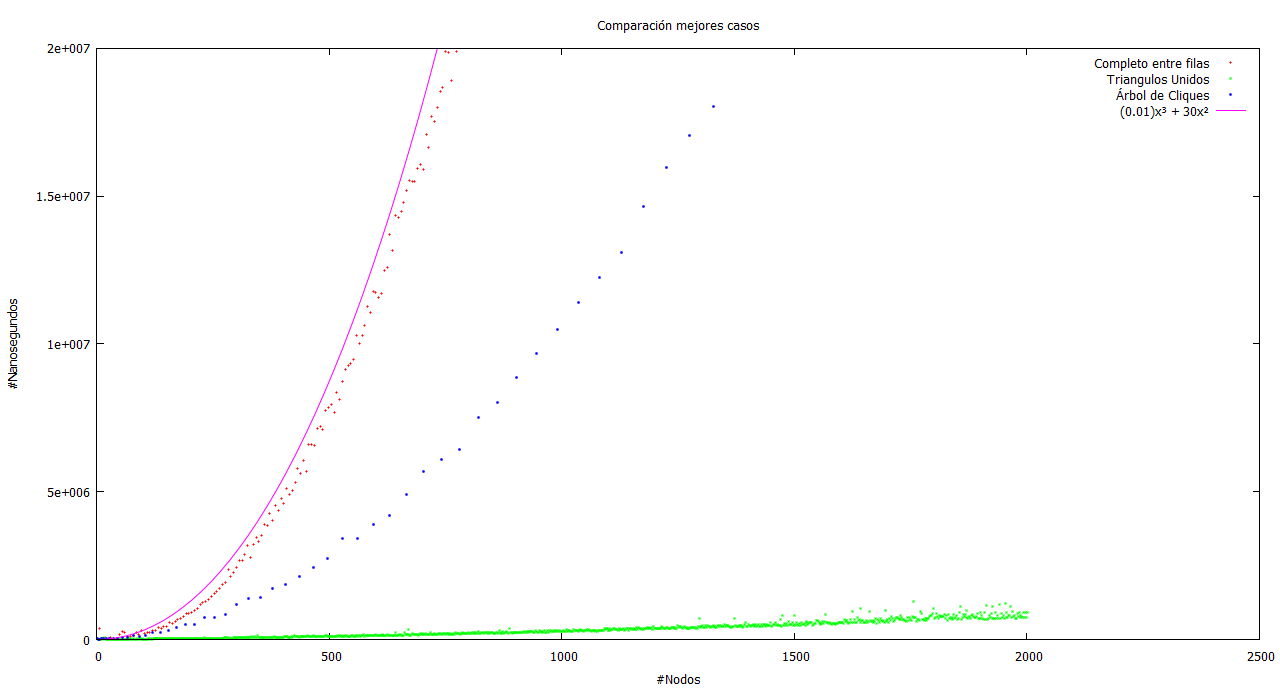
\includegraphics[width=17cm]{./graficos/goloso-mejorescasos.png}
% grafico.eps: 0x0 pixel, 300dpi, 0.00x0.00 cm, bb=50 50 410 302
\end {center} 

En el gráfico se puede observar que el comportamiento de cada familias es muy regular sin picos ni sobresaltos, por lo tanto, sumado principalmente a que siempre devuelve un conjunto dominante óptimo, concluimos que para este tipo de familias es muy recomendable usar este algoritmo polinomial, sin necesidad de optimizarlo o probar distintas estrategias y/o heurísticas.

\subsection{Peor Caso}

Al ser una heurística, en ciertos casos la solución no es la óptima que podría dar un algoritmo exacto, pero aún asi es correcta.
Los peores casos, donde se produce una diferencia en el tamaño de conjunto dominante respecto a la optima, se suelen dar en grafos en los que varios nodos tienen el mismo grado o hay pequeña diferencia, y esto es debido que para la elección del vertice dominante en cada iteración nos quedamos con el que mayor grado de nodos adyacentes no cubiertos tenga y si hay varios con esta misma característica puede pasar que el nodo seleccionado no sea conveniente a futuro para llegar a una solución óptima.

En los siguientes ejemplos de grafos se puede apreciar mejor:

\begin {center}
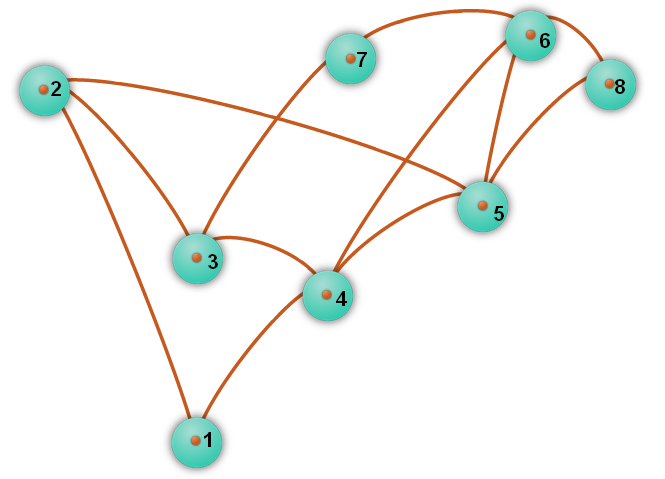
\includegraphics[width=8cm]{./graficos/grafo.png}
% grafico.eps: 0x0 pixel, 300dpi, 0.00x0.00 cm, bb=50 50 410 302
\end {center} 
La solución optima proporcionada por el algoritmo exacto es {6,2}, mientras que el goloso devuelve {4,3,5}, ya que como los nodos 6,4 y 5 tienen el mismo grado, al momento de la elección se decide por el 4 provocando esta diferencia en el tamaño del conjunto con respecto a la solución óptima.

\begin {center}
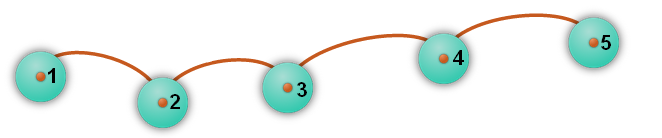
\includegraphics[width=8cm]{./graficos/grafo_camino.png}
% grafico.eps: 0x0 pixel, 300dpi, 0.00x0.00 cm, bb=50 50 410 302
\end {center} 
La solución óptima proporcionada por el algoritmo exacto es {2,4}, mientras que el goloso podría devolver {3,2,5}, ya que como los nodos 2, 3 y 4 tienen el mismo grado, si se decide por el 3, dejaría a todos los demás nodos con 1 grado sin dominar y faltando los dos extremos, provocando que si o si se necesite cubrirlos o elegirlos como dominantes, haciendo que el conjunto tenga tamaño 3 y no 2 como el exacto.

\subsubsection {Familias}
Las familias de grafos que encontramos que el algoritmo goloso da un resultado no optimo frente al exacto fue con los Möbius–Kantor y Grid. Esto suele pasar por que son regulares (3-regular) y casi regulares (4-regular internamente, 3-regular en los bordes) respectivamente y al momento de la elección del mejor vértice, la estrategia solo distingue por grado de adyacentes sin dominar por lo tanto seleccionará por el orden de la etiqueta de los nodos, las cuales son arbitrarias. 

\begin {center}
\includegraphics{./graficos/mobiusygrid.png}
% grafico.eps: 0x0 pixel, 300dpi, 0.00x0.00 cm, bb=50 50 410 302
\end {center} 

Considerando que Möbius–Kantor se puede reducir a un circuito con arcos, nos pareció mas interesante enfocarnos en los grafos Grid, ya que es más amplia la diferencia de resultados entre los dos algoritmos, además esta familia de grafos son de más utilidad, ya que equivalen tableros representando cada celda con un nodo.

La familia de grafos Grid se caracteriza principalmente por modelar un tablero en donde cada celda equivale a un nodo, y dos nodos son adyacentes si están en celdas contiguas. En base a los resultados de pruebas exactas con grandes cantidades de nodos$^{[2]}$, pudimos notar que la diferencia a las pruebas con nuestra heurísta se debe principalmente a que la estrategia seleccionará primero los nodos interiores por tener mayor grado sin dominar a su alrededor y luego completará con los bordes, siendo un grosero por el simple hecho de que con una óptima selección de nodos del borde al comienzo se podría $''$acorralar$''$ los nodos interiores necesitando una menor cantidad de estos para dominar todo el grafo. 

En la sección de \textbf{Cotas} se podrá observar que para este tipo de grafos, el tamaño del conjunto dominate esta por debajo de las cotas establecidas.

En el siguiente ejemplo, para un grafo Grid de 5x5 con 25 nodos, se puede notar la diferencia entre cantidad de elementos de los conjunto dominante resultantes, el goloso devuelve 9 nodos {6, 18, 21, 9, 1, 11, 20, 4, 23}, mientras que el exacto 7 nodos {19, 18, 10, 7, 4, 1, 21}, y esto se debe principalmente a que el goloso eligirá primero los nodos internos de grado 4 hasta que tengan el mismo grado sin dominar que los del borde y luego seleccionará los que faltan para dominar a todos, mientras que la solución exacta dependia más de los nodos en los bordes que los interiores.
 
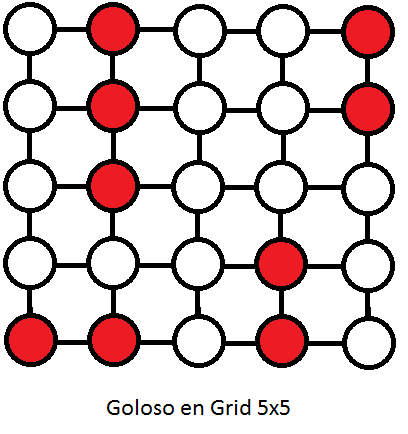
\includegraphics[width=8cm]{./graficos/grid_5x5_goloso.png}
% grafico.eps: 0x0 pixel, 300dpi, 0.00x0.00 cm, bb=50 50 410 302
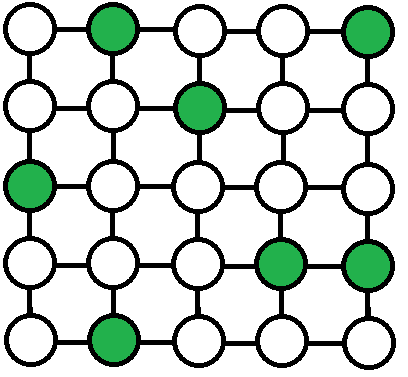
\includegraphics[width=8cm]{./graficos/grid_5x5_exacto.png}
% grafico.eps: 0x0 pixel, 300dpi, 0.00x0.00 cm, bb=50 50 410 302

Mediante varios casos de tests que fuimos corriendo y en comparativa con el  siguiente cuadro de valores para conjunto dominantes óptimos para grafos Grid$^{[2]}$, encontramos que la distancia entre los tamaño de la solución
del Greedy y del CDM puede ser bastante grande, por ejemplo, en el grafo de 29x29, con el goloso da soluciones de tamaño 248 cuando el óptimo es 188, con una diferencia de 60 nodos, bastante alto considerando que equivale a más de dos filas de nodos.\\

\begin {center}
\textbf{Tamaño de conjunto dominante óptimo para grafos Grid de tamaño n*m}
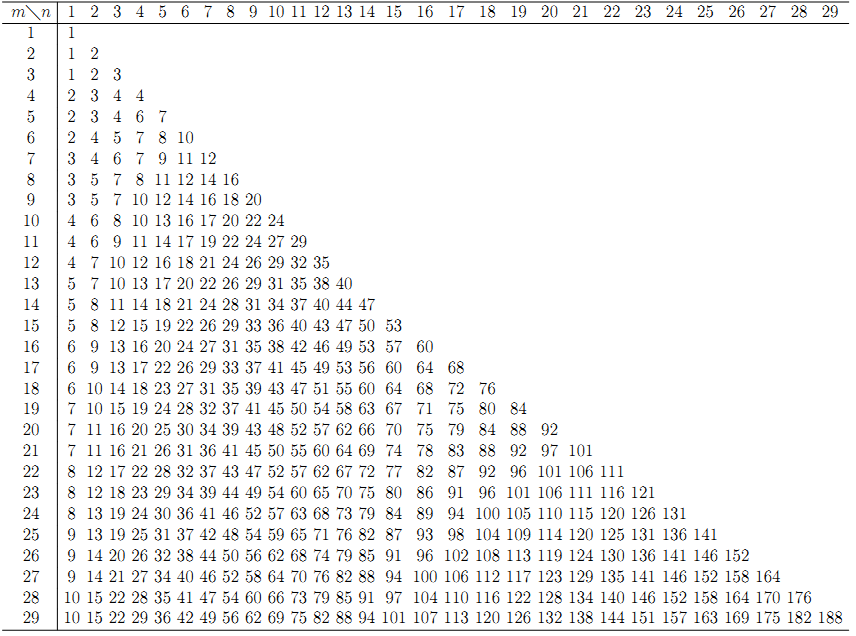
\includegraphics[width=18cm]{./graficos/cd_grid_exacto.png}
% grafico.eps: 0x0 pixel, 300dpi, 0.00x0.00 cm, bb=50 50 410 302
\end {center} 
\hbox{}
\begin {center}
\textbf{Tamaño de conjunto dominante goloso para grafos Grid de tamaño n*m}
\resizebox{18cm}{!} {
 \begin{tabular}{ l | l l l l l l l l l l l l l l l l l l l l l l l l l l l l l}
m / n & 1 & 2 & 3 & 4 & 5 & 6 & 7 & 8 & 9 & 10 & 11 & 12 & 13 & 14 & 15 & 16 & 17 & 18 & 19 & 20 & 21 & 22 & 23 & 24 & 25 & 26 & 27 & 28 & 29 \\ \hline
1 & 1 \\
2 & 1 & 2  \\
3 & 1 & 2 & 3  \\
4 & 2 & 3 & 4 & 6 \\
5 & 2 & 4 & 5 & 6 & 9  \\
6 & 2 & 4 & 6 & 8 & 10 & 10  \\
7 & 3 & 5 & 6 & 9 & 13 & 13 & 15  \\
8 & 4 & 5 & 8 & 12 & 12 & 16 & 15 & 21   \\
9 & 3 & 6 & 9 & 11 & 13 & 16 & 21 & 23 & 28   \\
10 & 4 & 7 & 10 & 14 & 15 & 19 & 20 & 27 & 28 & 30   \\
11 & 5 & 8 & 11 & 15 & 17 & 21 & 23 & 29 & 31 & 33 & 39   \\
12 & 6 & 8 & 11 & 16 & 17 & 21 & 26 & 31 & 34 & 36 & 43 & 45   \\
13 & 6 & 8 & 14 & 18 & 18 & 22 & 25 & 34 & 39 & 43 & 45 & 49 & 53   \\
14 & 6 & 9 & 14 & 16 & 21 & 23 & 28 & 34 & 39 & 43 & 49 & 51 & 54 & 57   \\
15 & 7 & 9 & 15 & 18 & 21 & 28 & 31 & 40 & 41 & 47 & 51 & 53 & 61 & 64 & 65   \\
16 & 7 & 10 & 16 & 19 & 22 & 31 & 32 & 40 & 45 & 51 & 54 & 59 & 63 & 67 & 69 & 80   \\
17 & 7 & 11 & 17 & 24 & 24 & 29 & 36 & 41 & 48 & 56 & 56 & 61 & 65 & 69 & 77 & 84 & 83   \\
18 & 6 & 11 & 18 & 24 & 25 & 33 & 37 & 40 & 50 & 58 & 61 & 64 & 69 & 76 & 81 & 87 & 89 & 95  \\
19 & 7 & 12 & 19 & 27 & 25 & 35 & 39 & 45 & 52 & 61 & 64 & 69 & 74 & 79 & 85 & 94 & 94 & 99 & 109   \\
20 & 8 & 12 & 19 & 28 & 29 & 35 & 41 & 46 & 53 & 62 & 66 & 73 & 77 & 84 & 90 & 97 & 94 & 106 & 112 & 119   \\
21 & 7 & 13 & 22 & 30 & 29 & 37 & 46 & 49 & 58 & 67 & 69 & 75 & 81 & 84 & 91 & 101 & 100 & 109 & 121 & 124 & 131\\
22 & 8 & 13 & 22 & 31 & 31 & 40 & 49 & 53 & 61 & 69 & 74 & 77 & 83 & 88 & 95 & 104 & 105 & 112 & 127 & 131 & 137 & 142 \\
23 & 9 & 13 & 23 & 33 & 31 & 38 & 51 & 56 & 64 & 71 & 76 & 83 & 90 & 93 & 97 & 109 & 110 & 119 & 133 & 139 & 139 & 153 & 158  \\
24 & 9 & 13 & 24 & 31 & 33 & 42 & 51 & 58 & 64 & 77 & 79 & 87 & 92 & 92 & 105 & 114 & 115 & 133 & 136 & 144 & 151 & 162 & 165 & 176  \\
25 & 9 & 14 & 25 & 33 & 36 & 42 & 53 & 57 & 66 & 76 & 80 & 87 & 96 & 100 & 108 & 118 & 119 & 133 & 142 & 149 & 158 & 163 & 169 & 180 & 182 \\
26 & 10 & 16 & 26 & 38 & 39 & 46 & 55 & 58 & 72 & 83 & 85 & 91 & 102 & 105 & 110 & 122 & 125 & 140 & 151 & 152 & 164 & 172 & 183 & 189 & 189 & 203  \\
27 & 10 & 16 & 27 & 38 & 43 & 45 & 56 & 60 & 71 & 83 & 89 & 97 & 107 & 110 & 114 & 126 & 129 & 141 & 156 & 157 & 166 & 177 & 183 & 197 & 200 & 217 & 217  \\
28 & 10 & 17 & 28 & 37 & 44 & 47 & 61 & 65 & 75 & 87 & 88 & 102 & 109 & 116 & 117 & 129 & 135 & 151 & 162 & 165 & 170 & 182 & 190 & 200 & 204 & 216 & 222 & 232 \\
29 & 11 & 18 & 29 & 40 & 40 & 51 & 59 & 68 & 78 & 78 & 94 & 106 & 114 & 120 & 121 & 139 & 139 & 156 & 170 & 183 & 179 & 189 & 192 & 213 & 211 & 219 & 232 & 245 & 248  \\
\end {tabular} 

}
\end {center} 

En base al tiempo de corrida para grafos Grid de 0 a 900 nodos, acotamos superiormente con una cubica ($0.27n^2 + 120n^2$) logrando una forma muy similar como se puede observar en el siguiente gráfico:
\begin {center}
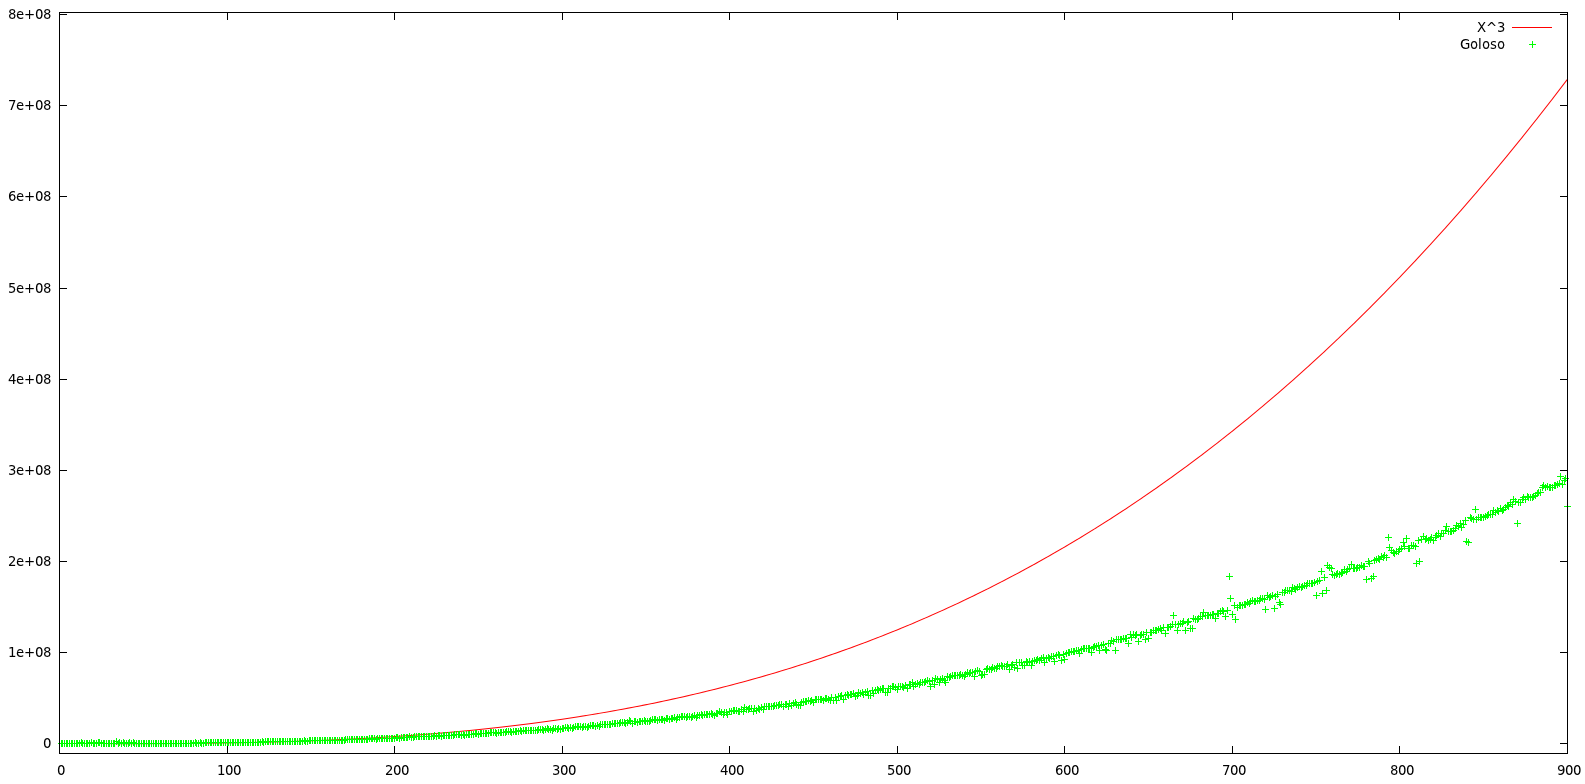
\includegraphics[width=19cm]{./graficos/goloso-900nodos.png}
% grafico.eps: 0x0 pixel, 300dpi, 0.00x0.00 cm, bb=50 50 410 302
\end {center} 

Por lo tanto se puede concluir que el algoritmo goloso no es recomendado para esta familia de grafos ya que, a pesar de tener complejidad polinomial cubica, a medida que aumenta la cantidad de nodos la diferencia aumenta considerablemente con respecto a la óptima 
